
%%%%%%%%%%%%%%%%%%%%%%%%%%%%%%%%%%%%%%%%%%%%%%%%%%%%%%%%
%
% Copyright (c) 2003-2010 by University of Queensland
% Earth Systems Science Computational Center (ESSCC)
% http://www.uq.edu.au/esscc
%
% Primary Business: Queensland, Australia
% Licensed under the Open Software License version 3.0
% http://www.opensource.org/licenses/osl-3.0.php
%
%%%%%%%%%%%%%%%%%%%%%%%%%%%%%%%%%%%%%%%%%%%%%%%%%%%%%%%%

\section{Newtonian Potential}

In this chapter we examine the gravitational potential field due to source
bodies and geological structure. The use of vector data and visualisation in
Mayavi is investigated.

The gravitational potential $U$ at a point $P$ due to a region with a mass
distribution $\rho(P)$ is given by Poisson's equation
\begin{equation} \label{eqn:poisson}
\nabla^2 U(P) = -4\pi\gamma\rho(P)
\end{equation}
where $\gamma$ is the gravitational constant.
If this is now related to the simplified general form
\begin{equation}
-\left(A\hackscore{jl} u\hackscore{,l} \right)\hackscore{,j} = Y
\end{equation}
where the LHS side is equivalent to 
\begin{equation} \label{eqn:ex10a}
-\nabla A \nabla u
\end{equation}
If $A=\delta\hackscore{jl}$ then equation \ref{eqn:ex10a} is equivalent to
\begin{equation*}
-\nabla^2 u
\end{equation*}
and thus Poisson's Equation \ref{eqn:poisson} satisfies the general form when
\begin{equation}
A=\delta\hackscore{jl} \text{ and } Y= 4\pi\gamma\rho
\end{equation}
At least one boundary point must be set for the problem to be solvable. For this
example we have set all of the boundaries to zero. The normal flux condition is
also zero by default. 

Setting the boundary condition is relatively simple using the \verb!q! and
\verb!r! variables of the general form, where
\begin{python}
q=whereZero(x[1]-my)+whereZero(x[1])+whereZero(x[0])+whereZero(x[0]-mx)
\end{python}
identifies the points on the boundary and \verb!r=0.0! sets the dirichlet
condition.

\section{Gravity Profile}
\sslist{example10a.py}

\begin{figure}[ht]
\centering
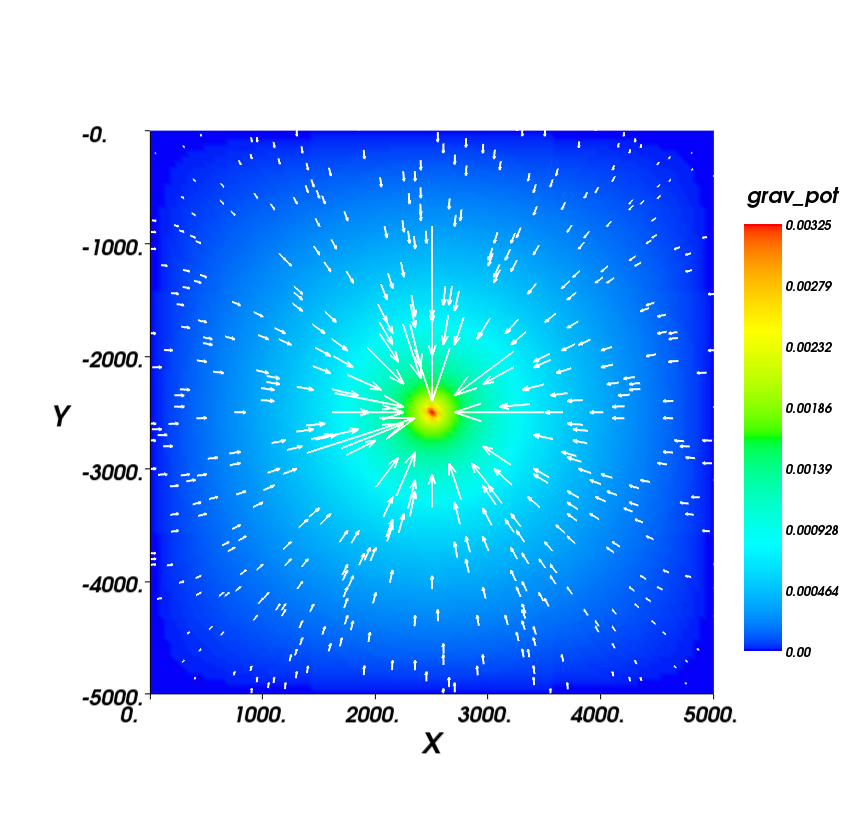
\includegraphics[width=0.75\textwidth]{figures/ex10apot.png}
\caption{Newtonian potential with g field directionality.}
\label{fig:ex10pot}
\end{figure}

\section{Gravity Well}
\sslist{example10b.py}

\begin{figure}[htp]
\centering
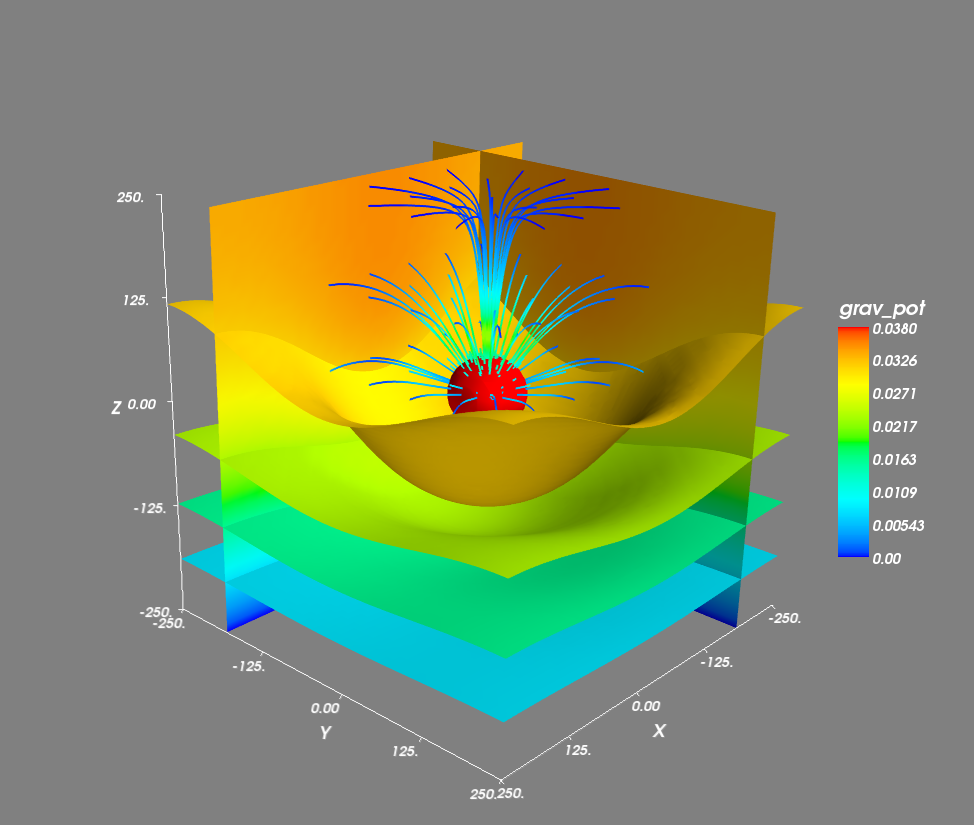
\includegraphics[width=0.75\textwidth]{figures/ex10bpot.png}
\caption{Gravity well with iso surfaces and streamlines of the vector
gravitational potential.}
\label{fig:ex10bpot}
\end{figure}

\section{Gravity Surface over a fault model.}
\sslist{example10c.py,example10m.py}
\begin{figure}[htp]
\centering
\subfigure[The geometry of the fault model in example10c.py.]
	{\label{fig:ex10cgeo}
	 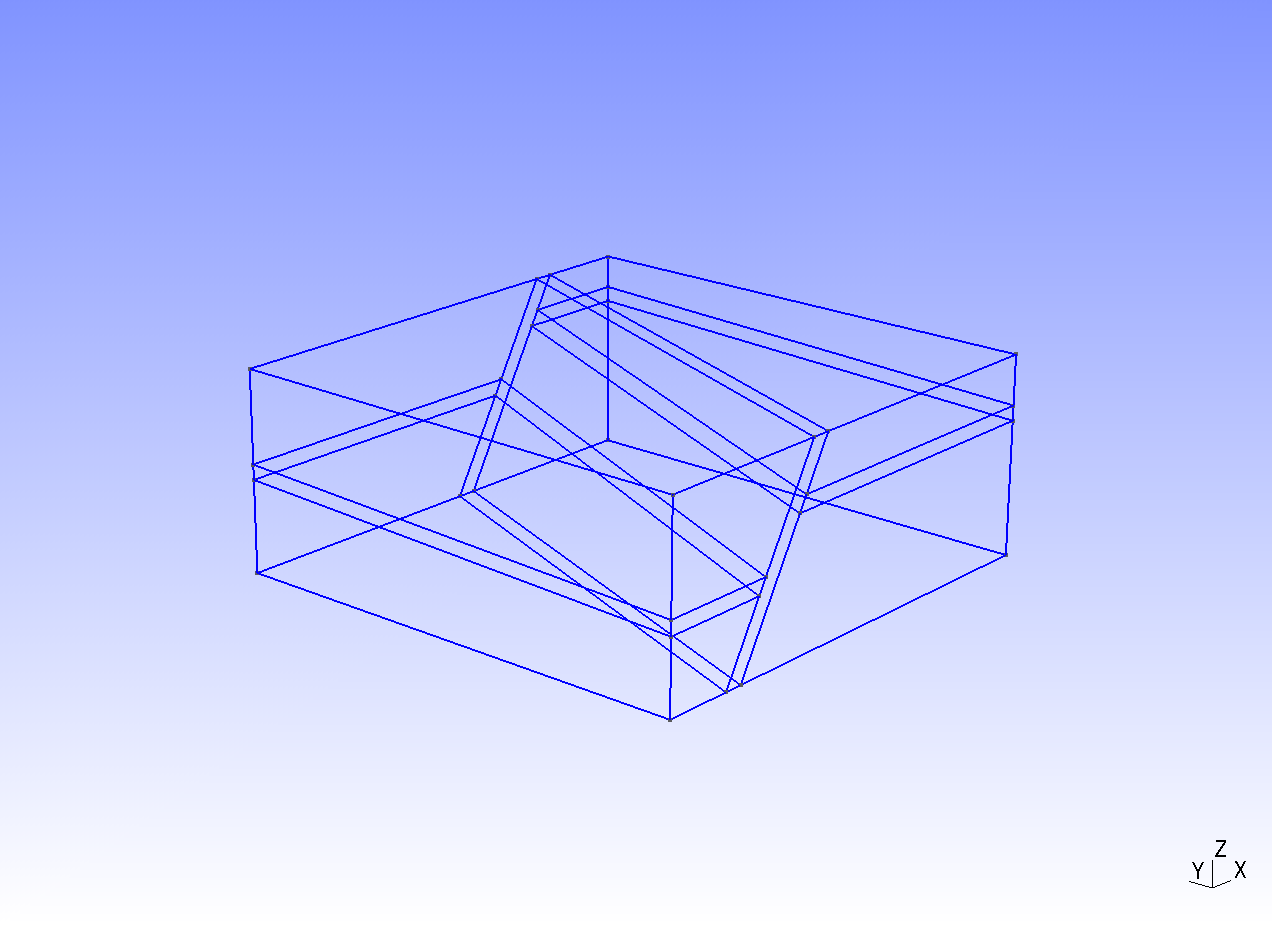
\includegraphics[width=0.8\textwidth]{figures/ex10potfaultgeo.png}} \\
\subfigure[The fault of interest from the fault model in
	example10c.py.] 
	{\label{fig:ex10cmsh}
	 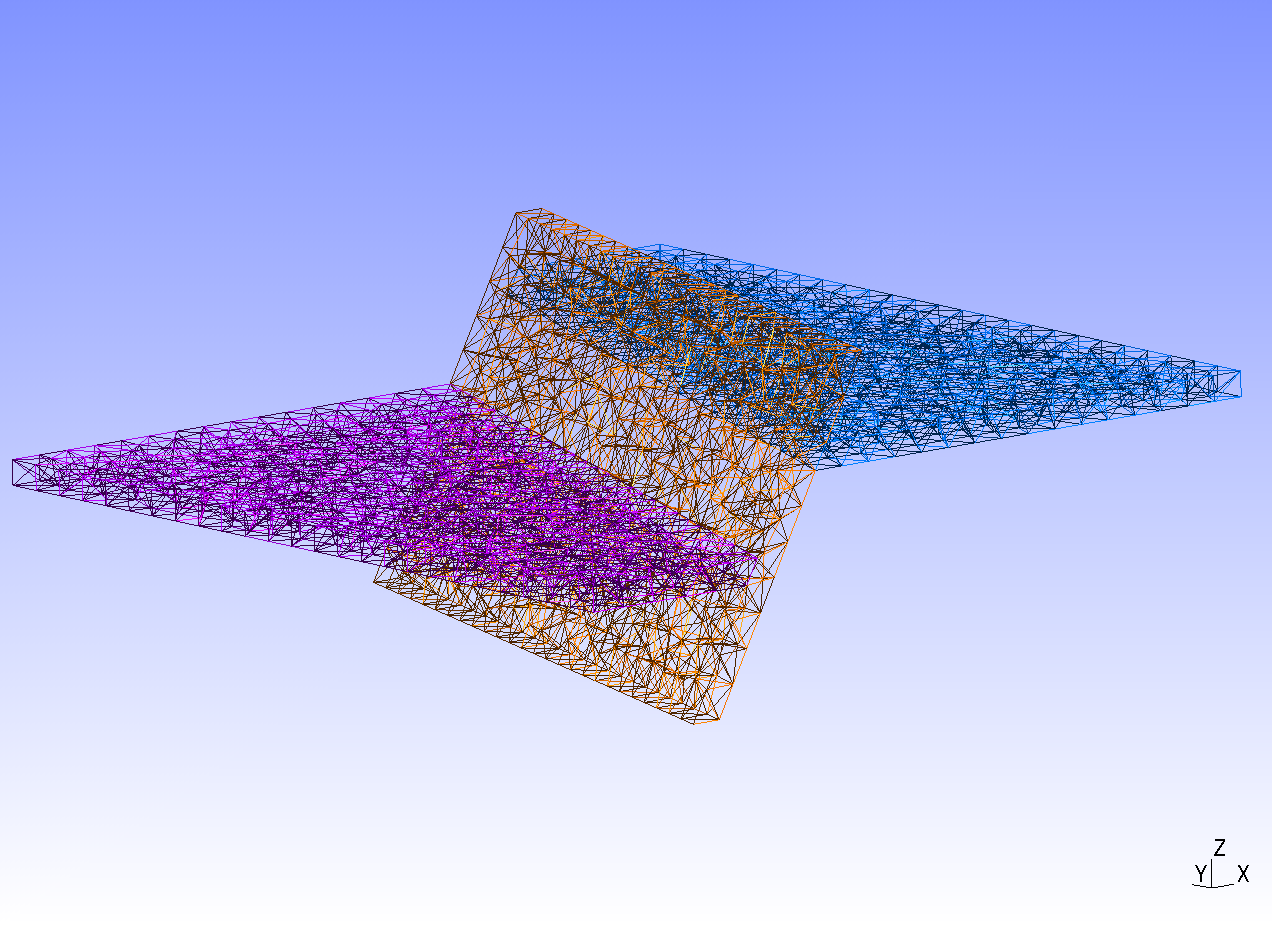
\includegraphics[width=0.8\textwidth]{figures/ex10potfaultmsh.png}}
\end{figure}

\begin{figure}[htp]
\centering
	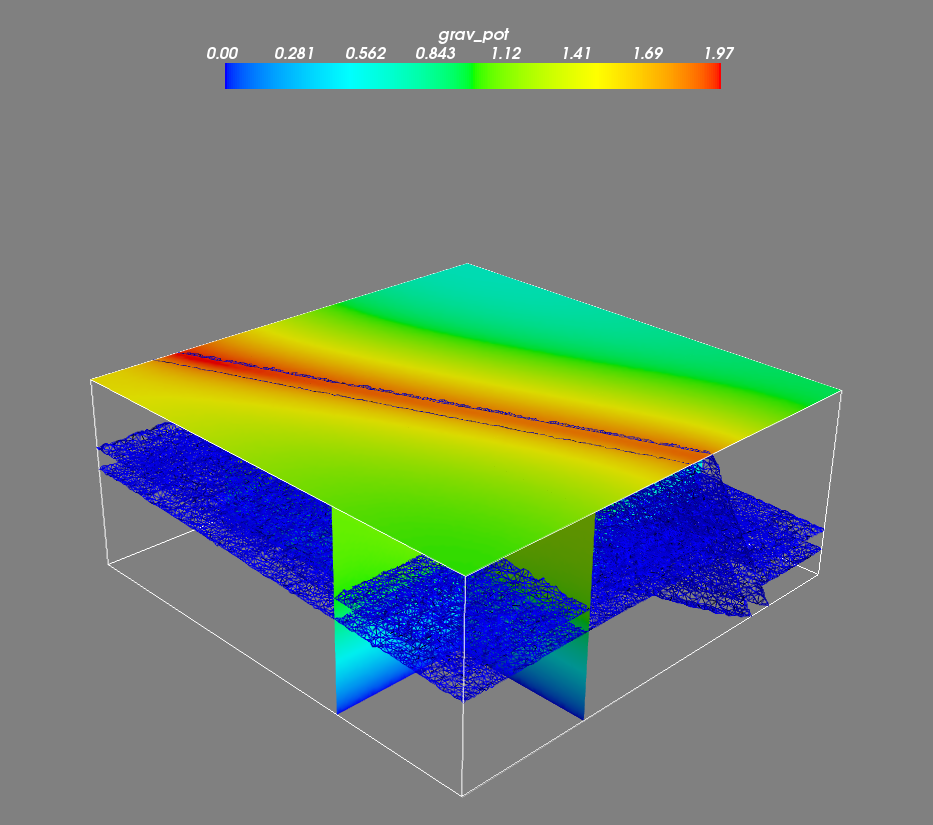
\includegraphics[width=0.8\textwidth]{figures/ex10cpot.png}
	\caption{Gravitational potential of the fault model with primary layers and
	faults identified as isosurfaces.}
	\label{fig:ex10cpot}
\end{figure}

